\documentclass[12pt]{report}

\title{A Mathematics Student's Lament}

\usepackage{authblk}

\author[1]{Nicholas Arvanitellis}
\author[2]{\\Jacob Bos}
\author[3]{\\Marcel Reverter-Rambaldi}

\affil[1,2,3]{Australian National University}
\affil[3]{The University of Queensland}



\usepackage{graphicx}
\usepackage{amsmath}
\usepackage{amssymb}
\usepackage{amsfonts}
\usepackage{amsthm}

\usepackage{float}

\usepackage{multicol}
\setlength{\columnsep}{1cm}

%\usepackage{setspace}

\usepackage[margin=2cm]{geometry}

\usepackage{xcolor}

\usepackage{titlesec}

\titleformat{\section}
{\color{purple}\normalfont\Large\bfseries}
{\color{purple}\thesection}{1em}{}

\titleformat{\subsection}
{\color{purple}\normalfont\bfseries}
{\color{purple}\thesubsection}{1em}{}

\titleformat{\subsubsection}
{\color{blue}\normalfont\bfseries}
{\color{blue}\thesubsubsection}{1em}{}


\begin{document}

    \maketitle
    \tableofcontents
\newpage


% ================================================================================================
% === Intro              =========================================================================
% ================================================================================================
\chapter{Introduction}




% ================================================================================================
% === Ch2 - The HSC ==============================================================================
% ================================================================================================
\chapter{The HSC}




% ================================================================================================
% === Ch3 - The SACE =============================================================================
% ================================================================================================
\chapter{The SACE}

\section{Stage 1}
\subsection{Essential Mathematics}

    According to the SACE subject outline, Stage 1 Essential Mathematics covers the following topics.
    \begin{table}[H]
        \centering
        \begin{tabular}{|l|l|}
        \hline
            1 & Calculations, time, and ratio \\ \hline
            2 & Earning and spending \\ \hline
            3 & Geometry \\ \hline
            4 & Data in context \\ \hline
            5 & Measurement \\ \hline
            6 & Investing \\ \hline
            7 & Open topic \\ \hline
        \end{tabular}
    \end{table}

\subsection{General Mathematics}

    According to the SACE subject outline, Stage 1 General Mathematics covers the following topics.
    \begin{table}[H]
        \centering
        \begin{tabular}{|l|l|}
        \hline
            1 & Investing and borrowing \\ \hline
            2 & Measurement \\ \hline
            3 & Statistical investigation \\ \hline
            4 & Applications of trigonometry \\ \hline
            5 & Linear and exponential functions and their graphs \\ \hline
            6 & Matrices and networks \\ \hline
            7 & Open topic \\ \hline
        \end{tabular}
    \end{table}

\subsection{Mathematics}

    According to the SACE subject outline, Stage 1 Mathematics covers the following topics.
    \begin{table}[H]
        \centering
        \begin{tabular}{|l|l|}
        \hline
            1 & Functions and Graphs \\ \hline
            2 & Polynomials \\ \hline
            3 & Trigonometry \\ \hline
            4 & Counting and Statistics \\ \hline
            5 & Growth and Decay \\ \hline
            6 & Introduction to Differential Calculus \\ \hline
            7 & Arithmetic and geometric series and sequences \\ \hline
            8 & Geometry \\ \hline
            9 & Vectors in the plane \\ \hline
            10 & Further Trigonometry \\ \hline
        \end{tabular}
    \end{table}


% ///////////////////////////////////////////////////////////////////////////////////////////////////
\section{Stage 2}
\subsection{Essential Mathematics}

    According to the SACE subject outline, Stage 2 Essential Mathematics covers the following topics.
    \begin{table}[H]
        \centering
        \begin{tabular}{|l|l|}
        \hline
            1 & Scales, plans, and models \\ \hline
            2 & Measurement \\ \hline
            3 & Business applications \\ \hline
            4 & Statistics \\ \hline
            5 & Investments and loans \\ \hline
            6 & Open topic \\ \hline
        \end{tabular}
    \end{table}

\subsection{General Mathematics}

    According to the SACE subject outline, Stage 2 General Mathematics covers the following topics.
    \begin{table}[H]
        \centering
        \begin{tabular}{|l|l|}
        \hline
            1 & Modelling with linear relationships \\ \hline
            2 & Modelling with matrices \\ \hline
            3 & Statistical models \\ \hline
            4 & Financial models \\ \hline
            5 & Discrete models \\ \hline
            6 & Open topic \\ \hline
        \end{tabular}
    \end{table}


\subsection{Mathematical Methods}

    According to the SACE subject outline, Stage 2 Mathematical Methods covers the following topics.
    \begin{table}[H]
        \centering
        \begin{tabular}{|l|l|}
        \hline
            1 & Further differentiation and applications \\ \hline
            2 & Discrete random variables \\ \hline
            3 & Integral calculus \\ \hline
            4 & Logarithmic functions \\ \hline
            5 & Continuous random variables \\ \hline
            6 & Sampling and confidence intervals \\ \hline
        \end{tabular}
    \end{table}

\subsection{Specialist Mathematics}

    According to the SACE subject outline, Stage 2 Mathematical Methods covers the following topics.
    \begin{table}[H]
        \centering
        \begin{tabular}{|l|l|}
        \hline
            1 & Mathematical induction \\ \hline
            2 & Complex numbers \\ \hline
            3 & Functions and sketching graphs \\ \hline
            4 & Vectors in three dimensions \\ \hline
            5 & Integration techniques and applications \\ \hline
            6 & Rates of change and differential equations \\ \hline
        \end{tabular}
    \end{table}

% ================================================================================================
% === Ch4 - The QCE =============================================================================
% ================================================================================================
\chapter{The QCE}





% ================================================================================================
% === ChX - What's Missing? ======================================================================
% ================================================================================================
\chapter{What's Missing?}




% ================================================================================================
% === ChY.1 - Stage 1 ============================================================================
% ================================================================================================
\chapter{An Alternative}

\begin{figure}[H]
    \centering
    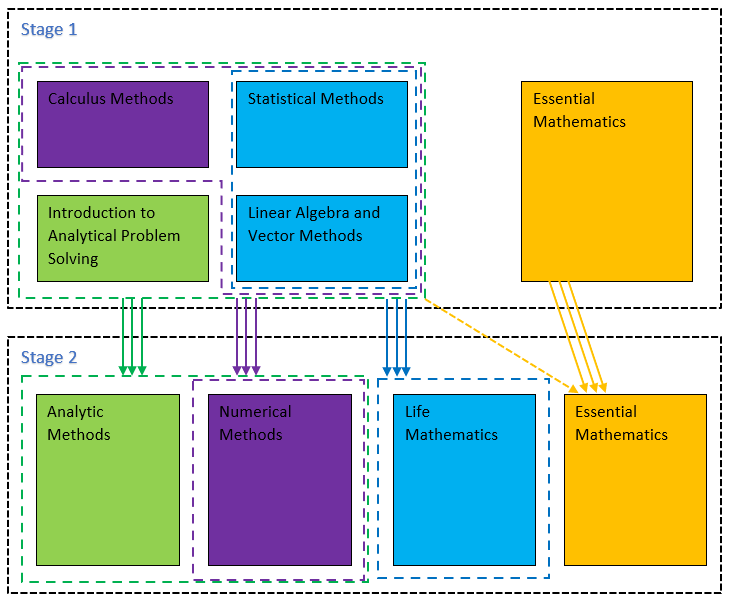
\includegraphics[width=0.8\textwidth]{Flowchart1.jpg}
    \caption{Subject structure}
\end{figure}

\section{Stage 1 - Year 11}

    \begin{table}[H]
        \centering
        \begin{tabular}{|l|l|}
        \hline
            S1.1 & The notion of probability and nPr/nCr Calculations \\ \hline
            S1.2 & Measures and Centre and Spread \\ \hline
            S2 & Continuous random variables \\ \hline
            S3 & Sampling, confidence intervals and hypothesis testing\\ \hline \hline \hline

            L1 & Geometric Trigonometry \\ \hline
            L2 & Vectors in the plane \\ \hline
            L3 & Matrices, networks and linear systems\\ \hline \hline \hline

            C1.1 & Functions and Graphs \\ \hline
            C1.2 & Polynomials \\ \hline
            C2.1 & Trigonometric functions \\ \hline
            C2.2 & Growth and Decay \\ \hline
            C3 & Introduction to Differential Calculus \\ \hline \hline \hline

            A1 & Geometry, Mathematical Problem Solving and Direct Proofs\\ \hline
            A2 & Sets, Elementary Set Operations and Relations\\ \hline
            A3 & Sequences, Series and Inductive Proofs\\ \hline
            AX & The map of mathematics\\ \hline
        \end{tabular}\\
        \caption{Main Cluster}
    \end{table}

\subsection{Essential Mathematics}
\subsection{Statistical Methods}
\subsection{Calculus Methods}
\subsection{Linear Algebra Methods}
\subsection{Introduction to analytic problem solving}

% ================================================================================================
% === ChY.2 - Stage 2 ============================================================================
% ================================================================================================
\section{Stage 2 - Year 12}

\subsection{Essential Mathematics}
\subsection{Life Mathematics}
\subsection{Analytical Methods}
    Analytical methods should serves to develop the analytical skills necessary for the mathematical, engineering and physical sciences and an appreciation of proof, logic and the fundamental structures of mathematics.

    Proposed topics are:
    \begin{table}[H]
        \centering
        \begin{tabular}{|l|l|}
        \hline
            1.1 & Logic and Proofs \\ \hline
            1.2 & Introduction to algebra and real analysis \\ \hline
            2 & Functions and graphs \\ \hline 
            3 & Polynomials and Complex numbers \\ \hline
            4 & Analytic Integration  \\ \hline 
            5.1 & Analytic solutions to differential equations \\ \hline
            5.2 & Vectors and Vector Calculus in three dimensions\\ \hline
        \end{tabular}
    \end{table}

    \subsubsection{Introduction to mathematics}
        \paragraph*{Logic and Proofs} (Including $\forall$, $\exists$, Negation, Direct, Contrapositive, Contradiction and Induction.)
        \paragraph*{Introduction to algebra and real analysis} ($\varepsilon - N$ and $\varepsilon - \delta$ limit definitions, groups, permutation groups, cyclic groups.)
    \subsubsection{Functions and Graphs} (with links to analysis)
    \subsubsection{Polynomials and Complex Numbers} (Lead from solutions to Polynomials to Complex numbers to realizing roots of unity as a cyclic group)
    \subsubsection{Analytic integration} (Parts, Substitution and inverse trigonometric functions)
    \subsubsection{Differential equations, vectors and vector calculus}
        \paragraph*{Analytic solutions to differential equations} (Separable DEs, harmonic oscillators and logistic growth)
        \paragraph*{Vectors and Vector Calculus in three dimensions} (Volume integrals, parametric curves, vector fields and partial differentiation)



\subsection{Numerical Methods}
    Numerical methods should serves to develop the topics learned in stage with emphasis on the computational skills necessary for engineering, computer science and sciences with an appreciation of computer driven calculation.

    Proposed topics are:
    \begin{table}[H]
        \centering
        \begin{tabular}{|l|l|}
        \hline
            1.1 & Introduction to computational approaches and the julia language\\ \hline
            1.2 & Revision of common differential functions\\ \hline
            2 & Further differentiation and applications \\ \hline
            3 & Integral calculus \\ \hline
            4 & Discretization of calculus models\\ \hline
            5 & Computational linear algebra \\ \hline
            6.1 & Statistics and computation \\ \hline
            6.2 & Computational problem solving \\ \hline
        \end{tabular}
    \end{table}

    \subsubsection{Introduction and revision} (Revise logarithmic, exponential and trigonometric functions) (Introduce for, while and recursive loops, digital boolean logic [and, or, if-then-else] introduce the motivation for using julia and appreciate the difference between scripting and repl based interface)
    \subsubsection{Further differentiation and applications} (Extend to differentiating trig, exponential and logarithmic functions as well as chain product and quotient rules)
    \subsubsection{Integral calculus} (FTOC, integrating trig, exponential and logarithmic functions)
    \subsubsection{Discretization of calculus models} (discrete differentiation, Midpoint rule, trapezoid rule, simpson's rule, simulating first order DEs like HOs)
    \subsubsection{Computational linear algebra} (Elementary rol ops, Solutions to systems of LEs with row reduction and cramer's rule, Shortest distance between planes and line problems in n dimensions, markov chains and steady states)
    \subsubsection{Further computation} 
        \paragraph*{Statistics and computation} (Application of previously learned statistics on large datasets. Dealing with .csv files etc... )
        \paragraph*{Computational problem solving} (Basic cellular automata, Monte-carlo methods, financial applications, reasoning on algorithmic complexity linear, quadratic, exponential)

\end{document}